\section{Theorie}

In dem folgenden Versuch soll mithilfe eines präziesen Verfahrens die Zeeman-Aufspaltung
von \ce{^{85}Rb} und \ce{^{87}Rb} untersucht werden. Das verwendete Verfahren wird
als optisches Pumpen bezeichnet.
Die Elektronenhülle eines isolierten Atoms besitzt diskrete Energieniveaus, wobei
die Nievaus der innersten Schalen vollständig mit Elektronen besetzt sind
(gemäß dem Pauli-Ausschlussprinzips). Für die äußeren Schalen ist bekannt, dass die
Niveaus mit einer höheren Energie schwächer besetzt sind. Zwei Niveaus
mit den Energien $W\ua{1}$ und $W\ua{2}$ ($W\ua{1}$ < $W\ua{2}$) und Besetzungszahlen
$N\ua{1}$ und $N\ua{2}$ sind gemäß der folgenden Relation miteinander verknüpft.

\begin{equation}
  \frac{N\ua{2}}{N\ua{1}} = \frac{g\ua{2}}{g\ua{1}} \frac{\exp{(-W\ua{2}/kt)}}{\exp{(-W\ua{1}/kt)}}
  \label{eqn:NRelation}
\end{equation}

Hierbei sind die $g\ua{i}$ die zugehörigen statistischen Gewichte.
Durch das Verfahren des optischen Pumpens kann nun eine Inversion der Besetzung
erzeugt werden,
bei der $N\ua{1}$ < $N\ua{2}$ gilt. Durch nachfolgende induzierte Strahlungsübergänge
kann die Energie der emittierten Quanten präzise ausgemessen werden. Somit lassen
sich durch Untersuchung der Zeeman-Aufspaltung verschiedene
Größen der Rubidium-Isotope bestimmt werden.

\subsection{Magnetische Momente}
\label{subsec:MagMo}

Sowohl der Bahndrehimpuls $\vec{L}$ als auch der Spin $\vec{S}$ besitzen
ein magnetisches Moment, welches Abhängig vom Betrag der Größe ($|\vec{L}|$ bzw.
$|\vec{S}|$), dem g-Faktor
und dem Bohrschen Magneton ist. Da die beiden Größen zu einem Gesamtdrehimpuls
$\vec{J}$ koppeln, kann dementsprechend auch ein magnetisches Moment $\vec{\mu}\ua{J}$
definiert werden.

\begin{align}
  |\vec{\mu}\ua{L}| &= \mu\ua{B} \sqrt{L(L+1)} \\
  |\vec{\mu}\ua{S}| &= g\ua{S} \mu\ua{B} \sqrt{S(S+1)} \\
  \implies & \vec{\mu}\ua{J} = \vec{\mu}\ua{L} + \vec{\mu}\ua{S} \\
  & |\vec{\mu}\ua{J}| = g\ua{J} \mu\ua{B} \sqrt{J(J+1)}
\end{align}

$\vec{\mu}\ua{J}$ führt dabei eine Präzessionsbewegung um die $\vec{J}$-Richtung
aus, wodurch der senkrechte Anteil im zeitlichen Mittel verschwindet und nur der
parallele Anteil eine Rolle spielt. Durch vektorielle
Betrachtung von $\vec{L}$, $\vec{S}$ und $\vec{J}$ lässt sich eine
Formel für $g\ua{J}$ bestimmen:

\begin{equation}
  g\ua{J} \approx \frac{3J(J+1)+S(S+1)-L(L+1)}{2J(J+1)}
  \label{eqn:LandeJ}
\end{equation}

Unter Einfluss eines äußeren Magnetfeldes ändern sich aufgrund der Wechselwirkung
mit dem magnetischen Moment die Energieniveaus. Da $\vec{mu}\ua{J}$ ebenfalls eine
Präzessionsbewegung um $\vec{B}$ ausführt, hat nur die zu $\vec{B}$ parallele
Komponente einen Einfluss auf die Energeiniveaus. Aufgrund der Richtungsquantelung
können die Energieniveaus nur ganzzahlige Vielfache von $g\ua{J}\mu\ua{B}B$
annehmen, verknüpft durch die Orientierungsquantenzahl $M\ua{J}$.

\begin{equation}
  U\ua{mag} = M\ua{J}g\ua{J}\mu\ua{B}B, \qquad M\ua{J} \in [-J,...,J]
  \label{eqn:EdiffJ}
\end{equation}

Die Energieniveaus spalten somit in $2J+1$ Unternivaus auf.

\subsection{Einfluss des Kernspins}
\label{subsec:Kern}

Beide Rubidium-Isotope besitzen einen Kernspin ungleich Null, weshalb eine
weitere Aufspaltung beachtet werden muss, die Hyperfeinstruktur.
Sie entsteht durch die Kopplung von Gesamtdrehimpuls und Kernspin:

\begin{equation}
  \vec{F} = \vec{J} + \vec{I}
\end{equation}

Die Quantenzahl $F$ läuft somit von $I+J$ bis $|I-J|$ und spaltet in $2J+1$ oder
$2I+1$, je nachdem ob $J<I$ oder $J>I$ ist. Wird hier zusätzliches
ein nicht zu hohes, äußeres Magnetfeld angelegt, spalten alle Hyperfeinstrukturniveaus
erneut in $2F+1$ Unterniveaus auf. Diese lassen sich charakterisiert durch die
Quantenzahl $M\ua{F}$ (siehe Abbildung \ref{fig:ZeemanKern}).
Die einzelnen Zeeman-Niveaus sind äquidistant mit folgender Energiedifferenz:

\begin{equation}
  U\ua{HF} = g\ua{F}\mu\ua{B}B.
  \label{eqn:EdiffF}
\end{equation}

\begin{figure}[h]
  \centering
  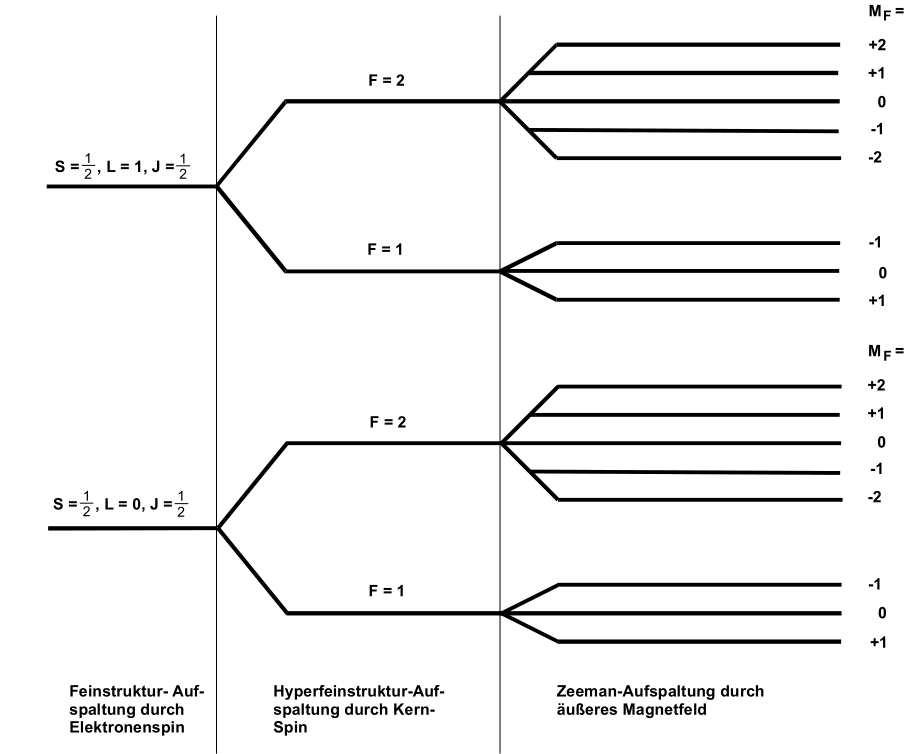
\includegraphics[width=\textwidth]{Pics/ZeemanKern.png}
  \caption{Hyperfeinstruktur und Zeeman-Aufspaltung bei einem Alkali-Atom
  mit Kernspin I = $\frac{3}{2}$. \cite{Anleitung}}
  \label{fig:ZeemanKern}
\end{figure}

Durch eine ähnliche Vektorenbetrachtung wie in Kapitel \ref{subsec:MagMo} lässt sich unter
Betrachtung von $|\mu\ua{F}| = \sqrt{F(F+1)}g\ua{F}\mu\ua{B}$ der entsprechende
Landé-Faktor bestimmen:

\begin{equation}
  g\ua{F} = g\ua{J} \frac{F(F+1)+J(J+1)-I(I+1)}{2F(F+1)}.
  \label{eqn:g_F}
\end{equation}

\subsection{Optisches Pumpen}
\label{subsec:OptP}

Wie in der Einleitung beschrieben, muss für die Vermessung der Zeeman-Niveaus erst
eine Inversion der Besetzungszahlen erzeugt werden. Im Folgenden wird zur Erklärung des
Prinzips die vereinfachende Annahme getroffen, dass das zu betrachtende Alkali-Atom
einen Kern mit verschwindenden Drehimpuls besitzt. Wird der Grundzustand \ce{^{2}S_{1/2}},
sowie die beiden ersten angeregten Zustände \ce{^{2}P_{1/2}} und \ce{^{2}P_{-1/2}}
betrachtet, ergibt sich das $\symup{D}_1-\symup{D}_2$-Dublett (siehe Abbildung \ref{fig:D1D2}).

\begin{figure}[h]
  \centering
  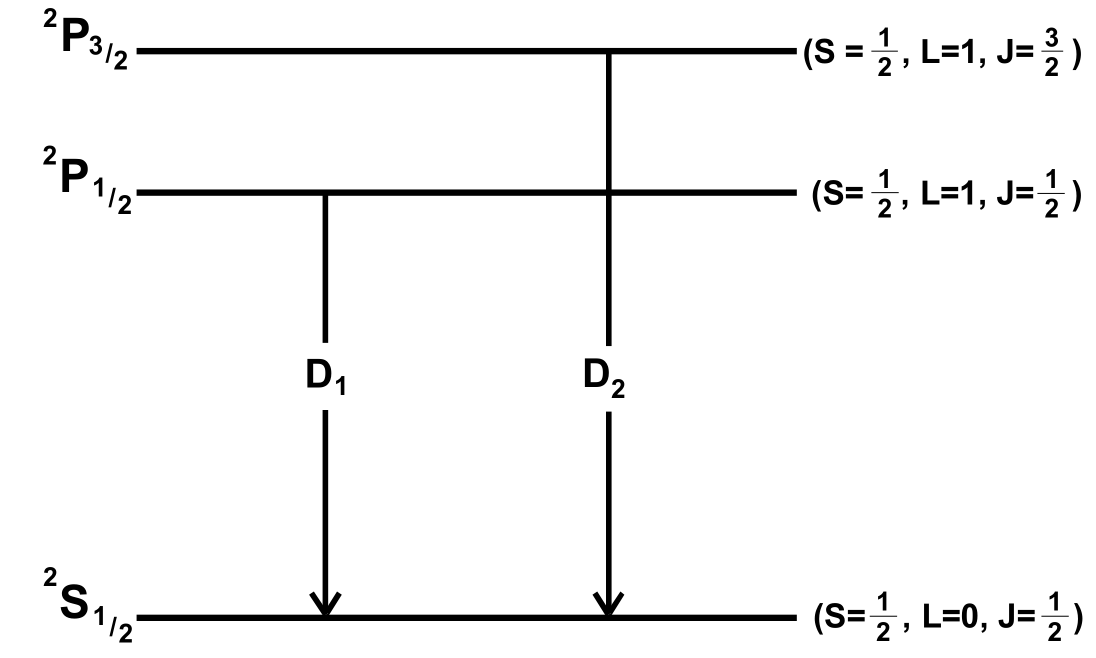
\includegraphics[width=\textwidth]{Pics/D1D2.png}
  \caption{Übergänge eines Alkali-Spektrums, bei denen D1- und D2-Licht emittiert
  werden. \cite{Anleitung}}
  \label{fig:D1D2}
\end{figure}

Bei allen Zuständen ist $J=\frac{1}{2}$, somit kann $M\ua{J}$ nur die Werte $+\frac{1}{2}$
oder $-\frac{1}{2}$ annehmen.
Jedes Niveau spaltet somit in zwei Zeeman-Unterniveaus auf (siehe Abbildung \ref{fig:Zeemanohne}).

\begin{figure}[h]
  \centering
  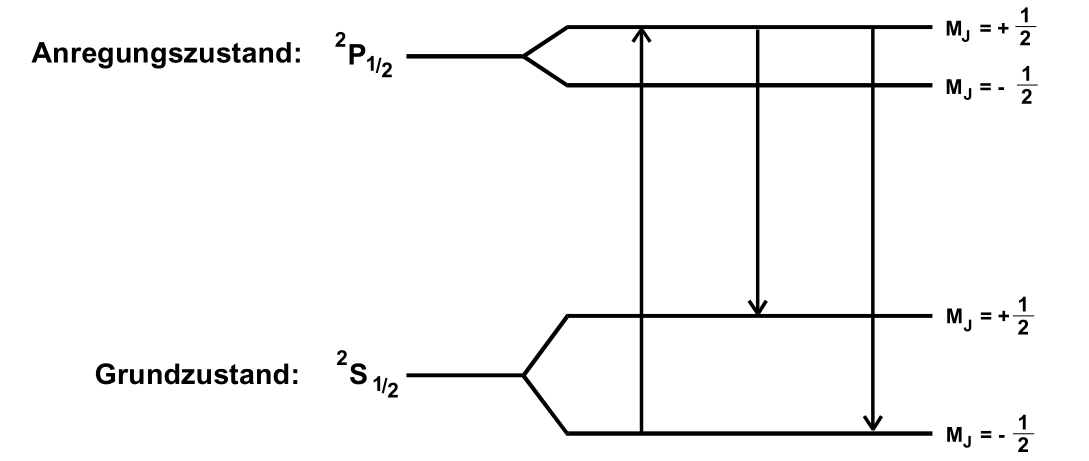
\includegraphics[width=\textwidth]{Pics/Zeemanohne.png}
  \caption{Zeeman-Aufspaltung bei einem Alkali-Atom ohne Kernspin, sowie die
  verschiedenen Übergänge. \cite{Anleitung}}
  \label{fig:Zeemanohne}
\end{figure}

Gemäß der Auswahlregeln für Strahlungsübergänge lassen sich 3 Übergänge unterscheiden,
die durch ihre Energie und ihren Polarisationszustand charakterisiert werden
(siehe Abbildung \ref{fig:Zeemanohne}).

\begin{enumerate}
  \item[a)] $\sigma^{+},\increment M\ua{J}=+1$: \\
    Das Licht ist rechtszirkular polarisiert, somit steht der Spin antiparallel
    zur Ausbreitungsrichtung.
  \item[b)] $\sigma^{-},\increment M\ua{J}=-1$: \\
    Das Licht ist linkszirkular polarisiert, somit steht der Spin parallel zur
    Ausbreitungsrichtung.
  \item[c)] $\pi, \increment M\ua{J}=0$: \\
    Das Licht ist linear polarisiert, parallel zu dem angelegten $\vec{B}$-Feld.
\end{enumerate}

Aufgrund des Dipolcharakters erscheinen die $\sigma$-Übergänge in allen zu $\vec{B}$
senkrechten Richtungen linear polarisiert.

Befindet sich in der Dampfkammer ein Gas aus den voher angesprochenen Alkali-Atome,
so kann mithilfe des optischen Pumpens eine Inversion der $M\ua{J}$ Niveaus des
$\ce{^{2}S_{1/2}}$ Zustandes erzeugt werden. Das $M\ua{J}=+\frac{1}{2}$ Niveau ist
anfangs schwächer besetzt als das $M\ua{J}=-\frac{1}{2}$ Niveau. Durch Einstrahlen
von $\symup{D}_1$-Licht werden nun $\increment M\ua{J} = +1$ Übergänge angeregt. Somit ist
lediglich der Übergang von $\ce{^{2}S_{1/2}}$ mit $M\ua{J}=-\frac{1}{2}$ zu $\ce{^{2}P_{1/2}}$ mit
$M\ua{J}=+\frac{1}{2}$ möglich. Durch spontane Emission geht der angeregte Zustand
nach ca. $10^{-8}$ s wieder in den Grundzustand über, wobei beide Niveaus
des Grundzustandes gleichwahrscheinlich bevölkert werden.
Aufgrund der Auswahlregel kann kein Übergang von $\ce{^{2}S_{1/2}}$ mit
$M\ua{J}=+\frac{1}{2}$ zu $\ce{^{2}P_{1/2}}$ mit $M\ua{J}=+\frac{1}{2}$ stattfinden,
wodurch sich die Besetzungen in diesem Niveau akkumulieren, während das $M\ua{J}=-\frac{1}{2}$ Niveau
entleert wird. Damit lässt sich theoretisch eine komplette Inversion der beiden Zustände erzeugen.
In der Realität ist es jedoch so, dass durch Zusammenstöße der Gasatome untereinander
die Elektronenspins umklappen können, so dass ein Übergang im Grundzustand vom
$M\ua{J}=+\frac{1}{2}$ Niveau zum $M\ua{J}=-\frac{1}{2}$ entsteht. Dies lässt sich
durch ein zusätzliches Puffergas in der Dampfkammer minimieren, wobei meistens ein
Edelgas gewählt wird.

Der Vorgang kann durch Beobachten der Intensität des am Ende der Dampfkammer
austretenden $\symup{D}_1$-Lichtes überprüft werden. Dafür wird ein Lichtdetektor hinter der
Zelle montiert (siehe Kapitel \ref{subsec:Aufbau}, Abbildung \ref{fig:Aufbau}).
Durch die Entleerung des $M\ua{J}=-\frac{1}{2}$
Niveaus wird mit der Zeit immer weniger Licht von dem Gas absorbiert, weswegen
die Transparenz der Kammer immer weiter zunimmt und sich asymptotisch der vollkommenen
Transparenz annähert (siehe Abbildung \ref{fig:Transparenz1}).

\begin{figure}[h]
  \centering
  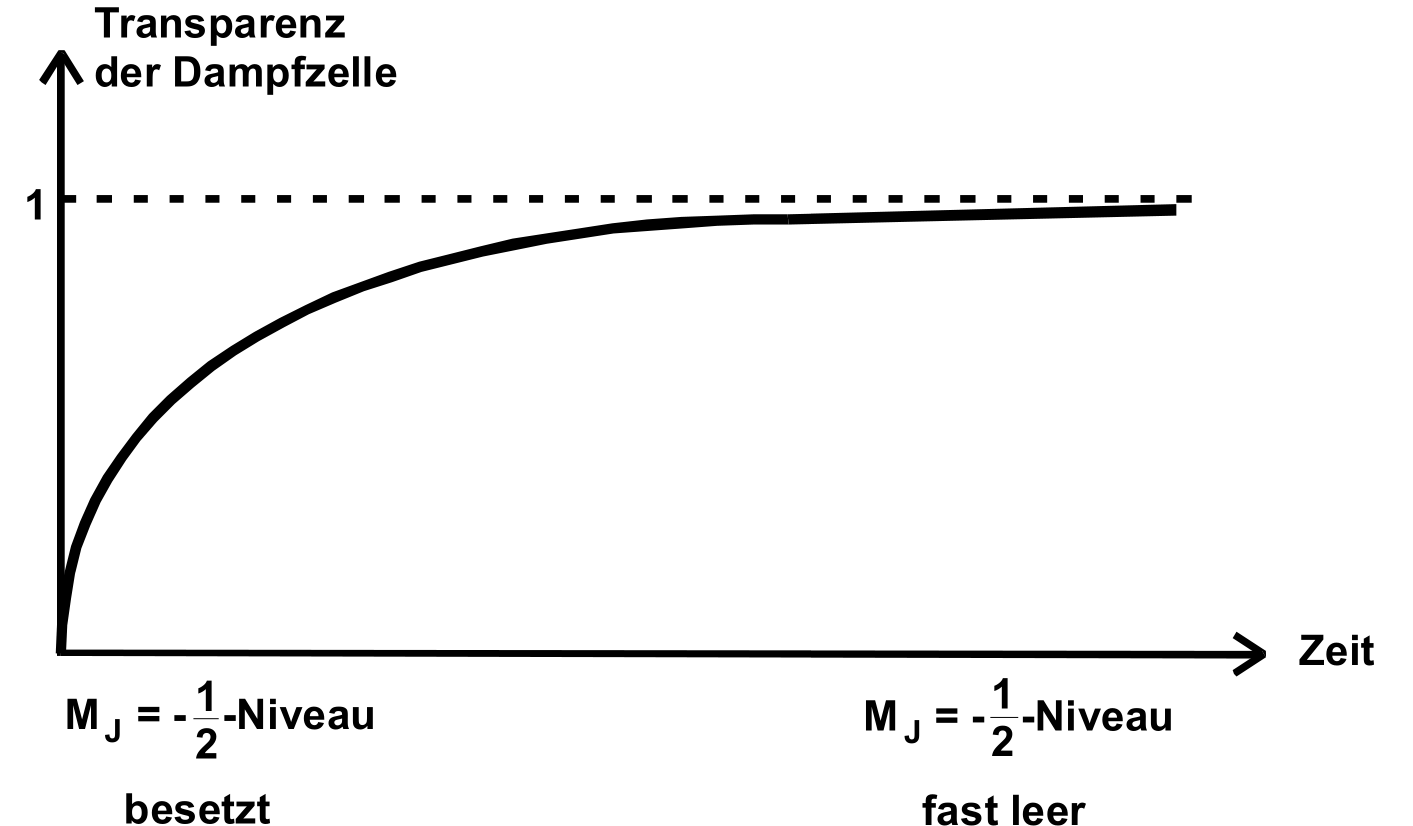
\includegraphics[width=\textwidth]{Pics/Transparenz1.png}
  \caption{Transparenz der Dampfzelle im Verlauf des optischen Pumpens bei
  rechtszirkular-polarisiertem Licht. \cite{Anleitung}}
  \label{fig:Transparenz1}
\end{figure}

\subsection{Präzisionsmessung der Zeeman-Aufspaltung}
\label{subsec:Praezission}

Im Allgemeinen kann bei dem Rückgang eines angeregten Atoms in den Grundzustand
zwischen zwei verschiedenen Prozessen unterschieden werden (siehe Abbildung
\ref{fig:Emission} a.) und b.) ). Bei der spontanen Emission
emittiert ein angeregtes Atom ohne äußere Einflüsse ein Photon und geht so in den
Grundzustand über. Bei der induzierten Emission wird von außen ein Lichtquant eingestrahlt,
welches als Energie genau die Energiedifferenz der beiden Niveaus besitzen muss.
Dadurch treten zwei Photonen aus, die genau die selbe Energie, Ausbreitungsrichtung
und Polarisation besitzen.

\begin{figure}[h]
  \centering
  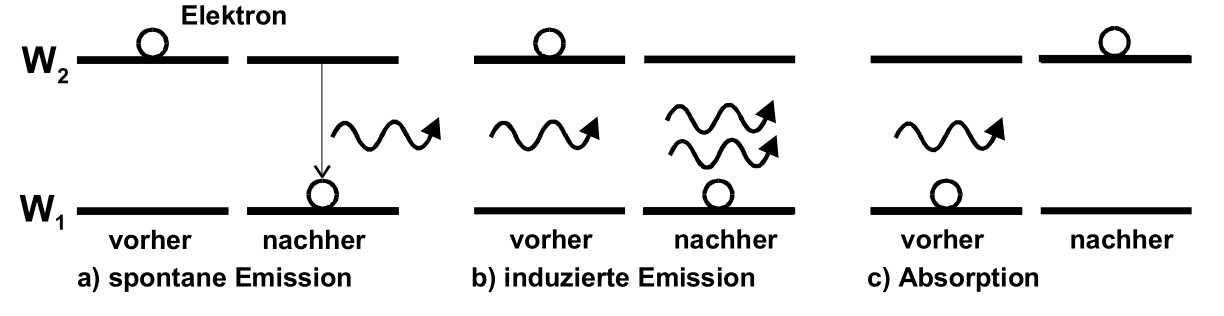
\includegraphics[width=\textwidth]{Pics/Emission.png}
  \caption{Verschiedene Übergangsmöglichkeiten zwischen zwei verschiedenen
  Energie-Niveaus. \cite{Anleitung}}
  \label{fig:Emission}
\end{figure}

Beide Prozesse laufen parallel ab, wobei der dominierende Prozess von der
Energie des emittierten Photons abhängt bzw. von der Frequenz, wie im Folgenden
nun hergeleitet wird.

\begin{equation}
  h\nu = W\ua{2} - W\ua{1}
  \label{eqn:Ediff}
\end{equation}

Nun wird ein Gas mit $N\ua{1}$ Atomen im Zustand $W\ua{1}$ und $N\ua{2}$
Atomen im energetisch höheren Zustand $W\ua{2}$ betrachtet, welches sich bei der
Temperatur $T$ im thermischen Gleichgewicht befindet. Die Anzahl der
spontanen Emissionen pro Zeiteinheit lässt sich dann wie folgt berechnen, wobei
$A\ua{21}$ die Übergangswahrscheinlichkeit von Niveau $W\ua{2}$ in $W\ua{1}$ darstellt:

\begin{equation}
  n\ua{spon} = N\ua{2}A\ua{21}.
  \label{eqn:Nspon}
\end{equation}

Die Anzahl induzierter Emissionen pro Zeiteinheit ist mit $N\ua{2}$ über den
Einstein-Koeffizienten $B\ua{21}$ sowie der Quantendichte $u(\nu)$ verbunden:

\begin{equation}
  n\ua{ind} = N\ua{2}B\ua{21}u(\nu).
  \label{eqn:Nind}
\end{equation}

Durch eine ähnliche Relation lässt sich auch die Anzahl absorbierter Quanten pro
Zeiteinheit bestimmen:

\begin{equation}
  n\ua{abs} = N\ua{1}B\ua{12}u(\nu).
  \label{eqn:Nabs}
\end{equation}

Da im thermischen Gleichgewicht die mittlere Besetzungszahl aller Zustände gleich
bleiben muss, muss die Anzahl emittierter Quanten in Summation gleich der Anzahl
absorbierter Quanten sein. Unter der Annahme, dass beide Niveaus nicht entartet
sind ($g\ua{1}=g\ua{2}$), gilt $B\ua{12} = B\ua{21}$. Somit lässt sich nun
$A\ua{21}$ bestimmen, so dass sich folgende Abhängigkeit ergibt:

\begin{equation}
  A\ua{21} = \frac{8\pi h}{c^3}B\ua{12}\nu^3.
  \label{eqn:A21}
\end{equation}

$B\ua{21}$ kann aufgrund seiner ausschließlichen Abhängigkeit von der Gestalt der
Wellenfunktionen als konstant betrachtet werden. Somit wird in Formel \eqref{eqn:A21}
aufgrund der $\nu^3$ Abhängigkeit deutlich, dass spontane Emission nur bei hohen
Frequenzen ein relevanter Prozess ist. Um dies deutlich zu machen, kann die
Übergangswahrscheinlichkeit für spontane Emission bei Rubidium betrachtet werden.
Für das Verhältniss der Übergangswahrscheinlichkeiten zwischen angeregtem Zustand
und Grundzustand ($\nu$
$\approx$ 380 THz) sowie dem Übergang zwischen zwei Zeeman-Niveaus ($\nu$
$\approx$ 1 MHz) ergibt sich $A\ua{21}(380\,THz)/A\ua{21}(1\,MHz)=5.4\cdot10^25$.
Somit ist die induzierte Emission im Bereich der Zeeman-Aufspaltung der dominierende
Prozess.

Mit den obigen Überlegungen lassen sich die Abstände zwischen den Zeeman-Niveaus
unter Verwendung der induzierten Emission präzise vermessen. Liegt zu Beginn noch
kein Magnetfeld an, so ist das optische Pumpen nicht möglich und die Transparenz
der Dampfkammer liegt ungefähr bei 0. Im Allgemeinen ist diese jedoch
aufgrund des Magnetfeldes der Erde nicht der Fall, wodurch sich dieses anhand der
Abweichung bestimmen lässt (siehe Abbildung \ref{fig:Transparenz2}).
Dafür kann durch Kompensations mittels eines
vertikalen Ausgleichsfeldes die Linienbreite minimiert werden.

\begin{figure}[h]
  \centering
  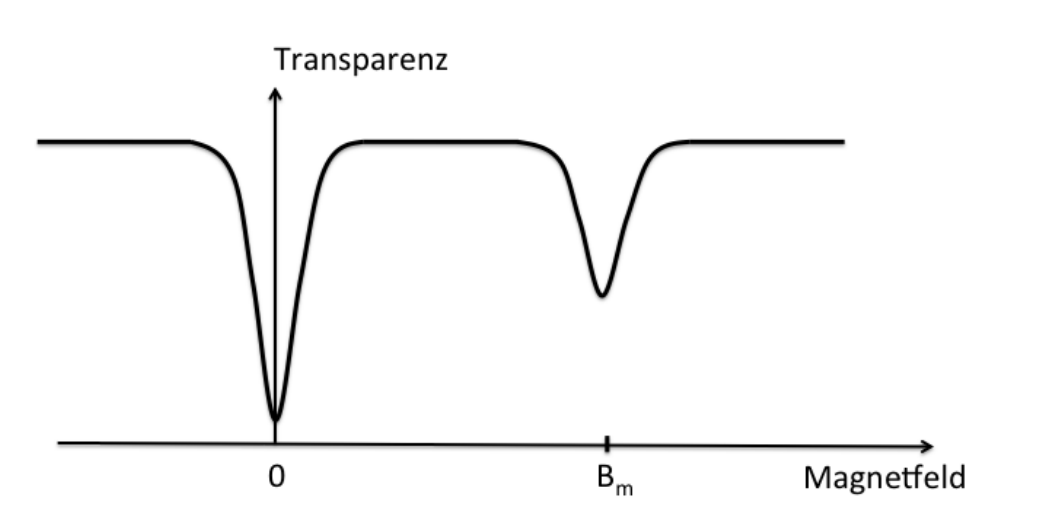
\includegraphics[width=\textwidth]{Pics/Transparenz2.png}
  \caption{Transparenz der Dampfzelle in Abhängigkeit von der angelegten Feldstärke.
   \cite{Anleitung}}
  \label{fig:Transparenz2}
\end{figure}

Außerhalb der Dampfzelle wird ein frequenzvariables Hochfrequenzfeld (weiter RF)
angelegt, womit später die induzierte Emission hervorgerufen wird. Aufgrund der
durch \ref{eqn:NuB} gegebenen Relation kann der Wert des anderen horizontalen
Magnetfeldes bestimmt werden,
bei dem durch das angelegte RF mit der festen Frequenz $\nu$ induzierte Emission
auftritt:

\begin{align}
  h\nu &= g\ua{J}\mu\ua{B}B\ua{m}\increment M\ua{J}
  \label{eqn:NuB} \\
  B\ua{m} &= \frac{4\pi m\ua{0}}{e\ua{0}g\ua{J}}\nu.
  \label{eqn:Bm}
\end{align}

Durch die auftretende Emission wird das $\ce{^{2}P_{1/2}}$,$M\ua{J}=+\frac{1}{2}$
wieder entleert und das D1-Licht kann wieder absorbiert werden. Die Transparenz
der Dampfzelle nimmt also im Resonanzfall wieder ab und die Magnetfeldstärke $B\ua{m}$
kann am Generator abgelesen werden (siehe Abbildung \ref{fig:Transparenz2}).

Die Hochfrequenz-Spektroskopie ermöglicht dabei diesen Versuch erst, da mit rein
optischen Methoden aufgrund der Begrenzung des Auflösungsvermögens die
Zeeman-Aufspaltung nicht anhand der Energieänderung der emittierten Lichtquanten
messbar ist.

Wird das angesprochene Verfahren auf ein Atom mit Kernspin $I > 0$ verallgemeinert,
so treten grunsätzlich keine neuen Phänomene auf. Lediglich die Aufspaltung wird
aufgrund der in Kapitel \ref{subsec:Kern} angesprochenen Kopplung verstärkt.
Anhand von Abbildung \ref{fig:ZeemanKern} wird zum Beispiel deutlich, dass durch
optisches Pumpen keine Emission von $F$=2,$M\ua{F}$=+2 im Grundzustand in einen
angeregten Zustand möglich ist, da kein Niveau mit $M\ua{F}$=+3 vorhanden ist.
Die Besetzungszahl dieses Niveaus würde also durch optisches Pumpen zunehmen. Also
kann auch in diesem Fall durch zirkular-polarisiertes eine Inversion erzeugt werden.
Ebenso lässt sich mittels der RF-Quanten wieder induzierte Emission erzeugen um
den Zeeman-Übergang anschließend zu vermessen.

\subsection{Quadratischer Zeeman-Effekt}
\label{subsec:Zeeman2}

Bei einer Erhöhung der Flussdichte des Magnetfeldes müssen bei Berechnung der
Energiedifferenz zwischen zwei Zeeman-Niveaus noch Terme höherer Ordnung
betrachtet werden. Durch Lösen der Schrödinger-Gleichung des vorhandenen Systems
ergibt sich für die Energie $U\ua{HF}$ noch ein zusätzlicher Term, welcher
propotional zu $B^2$ ist:

\begin{equation}
  U\ua{HF} \approx g\ua{F}\mu\ua{B}B + g\ua{F}^2\mu\ua{B}^2B^2 \frac{(1-2M\ua{F})}{\increment E\ua{Hy}}.
  \label{eqn:Uneu}
\end{equation}

$\increment E\ua{Hy}$ ist hierbei die Hyperfeinstrukturaufspaltung zwischen zwei
verschiedenen Niveaus. Somit ist die Zeeman-Energie hier auch von der Quantenzahl
$M\ua{F}$ abhängig, weswegen die vorliegenden Übergänge unterschiedliche
Energien besitzen (quadratischer Zeeman-Effekt).

\section{Aufbau und Durchführung}
\label{sec:AD}

\subsection{Aufbau}
\label{subsec:Aufbau}

\begin{figure}[h]
  \centering
  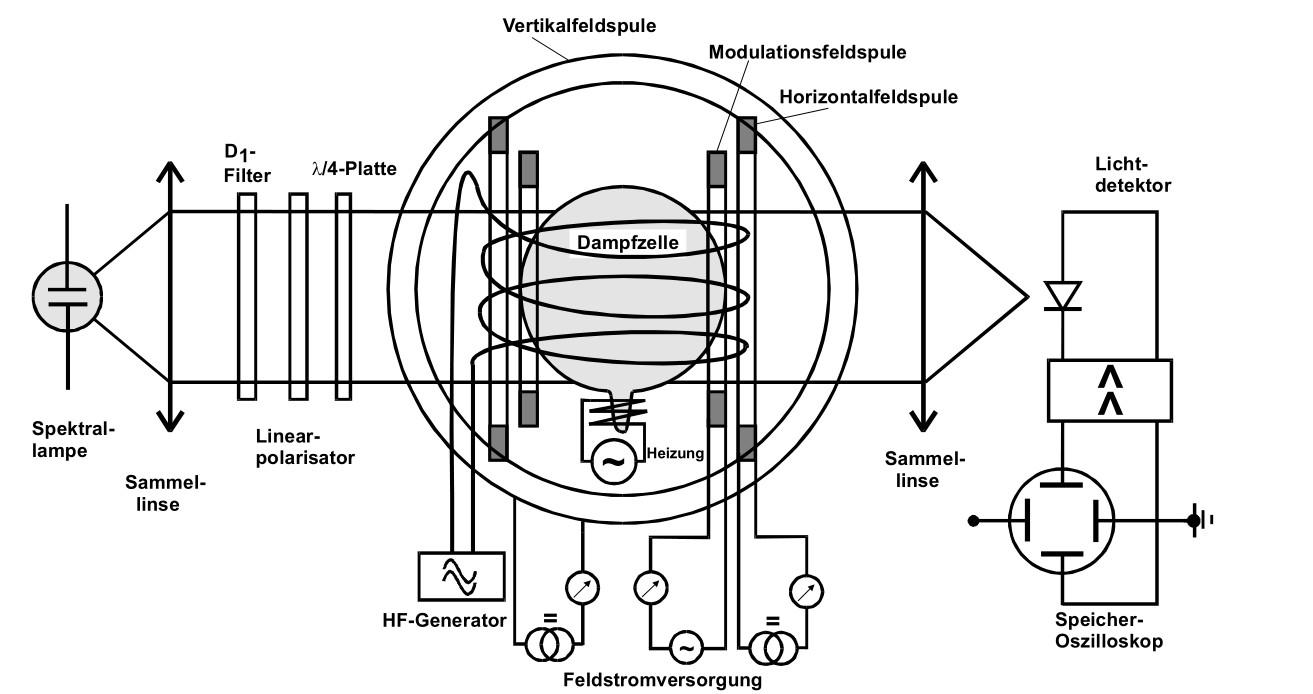
\includegraphics[width=\textwidth]{Pics/Aufbau.png}
  \caption{Aufbau der verwendeten Apparatur. \cite{Anleitung}}
  \label{fig:Aufbau}
\end{figure}

In Abbildung \ref{fig:Aufbau} ist die verwendete Apparatur dargestellt. Als Lichtquelle
wird hier ein mit Rubidium-Gas befüllte Spektrallampe verwendet. Das erzeugte Licht
wird mithilfe einer Sammellinse kollimiert, sodass anschließend mithilfe eines
Filters das $\symup{D}_1$-Licht heraussepariert wird. Durch einen Linearpolarisator sowie
ein $\frac{\lambda}{4}$-Plättchen wird das Licht dann zirkular-polarisiert.
Die Dampfzelle wird durch einen Ofen geheizt, damit ein optimaler Rb-Dampfdruck
herrscht. Mittels einer weiteren Linse hinter der Dampfkammer wird das austretende
Licht auf ein SI-Photoelement fokussiert, welches mit einem Oszilloskop augewertet
wird. Sichtbar werden die Schwankungen der Intensität durch eine Y-Auslenkung des
Elektronenstrahles.

Wie schon in Kapitel \ref{subsec:Praezission} beschrieben, werden bei dem Aufbau
drei Helmholtz-Spulenpaare verwendet. Zwei der Spulen sind Horizontal ausgerichtet
und eine Vertikal. Die Horizontalfeld-Spule besitzt $N = 154$ Windungen und hat einen
Radius von $R = 15.79\, \su{cm}$. Die Sweep-Spule (ebenfalls horizontal) besitzt einen
Radius von $R = 16.39\, \su{cm}$ sowie $N = 11$ Windungen je Spule. Die Vertikalfeld-Spule
besitzt $N=20$ Windungen sowie einen Radius von $R = 11.735\, \su{cm}$.

Alle drei Spulen können separat über ein Kontrollgerät gesteuert werden, an dem
auch die für das Sweep-Feld nötigen Werte (Startwert, Range und Dauer) eingestellt
werden können. Sweep- und Vertikalfeld-Spule besitzen einen maximalen Spulenstrom
von $I=1\,\su{A}$, welcher in $0.1\, \su{A}$ Schritten variiert werden kann. Die
Horizontalfeldspule hat einen maximalen Spulenstrom von $I= 3\,\su{A}$, welcher in
$0.3\,\su{A}$ Schritten variiert werden kann.

Die Messaparatur wird so ausgerichtet, dass der Verlauf des Strahles parallel
zur Nord-Süd-Richtung ist. So muss lediglich die parallele Komponente des Erdmagnetfeldes
betrachtet werden, welche in der Auswertung leichter zu Berücksichtigen ist.

Um die Resonanzstelle zu bestimmen wird bei fester Frequenz am RF die Horizontalfeldspule
über das Sweep-Feld variiert und dabei die Transparenz der Dampfzelle
mithilfe des Oszilloskopes beobachtet. Da die Reichweite des Sweep-Feldes jedoch
nicht komplett ausreicht, wird bei Frequenzen ab ca. 300 Hz ein zusätzliches
Horizontalfeld (Modulationsfeld) hinzugeschaltet. Das an der Photozelle
eintreffende Licht wird dann
am Oszilloskop per XY-Betrieb in Abhängigkeit der Sweep-Feldstärke dargestellt,
um die Resonanzstellen sichtbar zu machen.

\subsection{Durchführung}
\label{subsec:Durchführung}

Zu Beginn des Versuchs muss die Apparatur justiert werden. Vor der Justierung
der optischen Elemente werden "Gain", "Gain Multiplier" sowie "Meter Multiplier"
auf 1 gesetzt und die Zeitkonstante auf 100 ms eingestellt.
Danach werden unter Beobachtung der
Signalstärke am Galvanometer die beiden Linsen auf der Schiene verschoben, bis
die Signalstärke maximiert ist. Nach Einsetzen der restlichen optischen Elemente
wird der Aufbau mit einem Tuch abgedeckt..

Auf dem Oszilloskop kann anschließend der in Kapitel
\ref{subsec:Praezission} beschrieben Verlauf der Transparenz sichtbar gemacht
werden. Die Einstellungen der verschiedenen Felder sind im Folgenden listenförmig
dargestellt:

\begin{itemize}
  \item Potenziometer für alle Felder (beim Sweep-Feld der Startwert) werden auf
  Null gedreht.
  \item Unteren Schalter bei der Sweep-Spule auf "Continuous", oberen auf "Start"
  setzen und als Periodendauer 2 Sekunden einstellen.
  \item  "Recorder"-Ausgang der Sweep-Spule an Kanal 1 und die Dioden-Spannung an
  Kanal 2 des Oszilloskopes anschließen und als Darstellungsmodus den XY-Betrieb
  wählen.
  \item Anschließend "Gain" auf 20, "Gain Multiplier" auf x10 und "Meter Multiplier"
  auf x2 stellen.
\end{itemize}

Der anschließend sichtbare breite Peak (siehe Kapitel \ref{subsec:Praezission}) wird
durch Einstellen des Vertikal-Feldes schmaler gemacht, um das Erdmagnet-Feld
auszugleichen. Danach wird der
Versuchsaufbau mithilfe eines Kompasses so ausgerichtet, dass der Strahlenverlauf
entlang der Nord-Süd-Richtung verläuft.

Im letzetn Abschnitt des Experimentes werden die Resonanzfeldstärken gemessen.
Dafür wird am RF eine Frequenz von 100 kHz eingestellt. Mithilfe des Oszilloskopes
wird ein Foto der sichtbaren Peaks aufgenommen, um hinterher das Isotopenverhältniss
bestimmen zu können. Danach werden in Intervallschritten von 100 kHz bis zu einer
Frequen von 1 MHz die Magnetfeldstärken der Sweep-Spule an den Resonanzpeaks bestimmt.
Dabei wird "RF Amplifier Gain" auf 2 gestellt und eine Spannung mit 100 kHz und einer
Amplitude von 4 V angelegt.

Bei Frequenzen ab 300 kHZ wird wie in Kapitel \ref{subsec:Aufbau} beschrieben
ein zusätzliches horizontales Feld eingeschaltet, um mit dem Sweep die Resonanzen
abdecken zu können.
